\section{Convergence of CMA-ES with various step-size adaptations}
\subsection{Compared methods}

In this section we investigated rates of convergence and computing overhead of proposed methods. 
As mentioned in previous sections we considered five methods using different $\sigma$ adaptation rules:
  \begin{enumerate}
    \item CMA-ES-CSA
    \item CMA-ES-MSR
    \item CMA-ES-EXPTH
    \item CMA-ES-JA
    \item CMA-ES-QUANT
  \end{enumerate}

Each method used default settings for hyperparameters execpt for as mentioned above. All methods generated $\lambda = 4N$ points in each iteration.
For CMA-ES-MSR to count $K_{succ}$ of better points in current population than $j$-th best point of the previous population we set $j$ as:

\begin{equation*}
j = 0.3\lambda.
\end{equation*}

\subsection{Fitness functions: linear, quadratic, gutter}

To illustrate and compare rates of convergence we used two different fitness landscapes i.e. linear (\ref{eq:1}), quadratic
(\ref{eq:2}).

\begin{align}
  f_{l}(\wek{x}) &= x_{1}  \label{eq:1} \\
  f_{q}(\wek{x}) &= \sum^{D}_{i = 1} x^{2}_{i} \label{eq:2} \\
\end{align}

To assess the rates of convergence, each function was treated in as a minimalization problem and we recorded the fitness of the best point in the population. \\
The curves depicted in the figures below for iteration $t$ show the fitness of the best point and midpoint in the $t$th generation. \\ 
For each problem and algorithm, the mean point of population is initialized as:
\begin{equation*}
  \wek{m}_{i} = [100, \dots, 100]^{D}.
\end{equation*}

\subsection{Conclusions: convergence rate, benefits from using midpoint, search space dimension}

\begin{figure}[H]
\subfloat[]{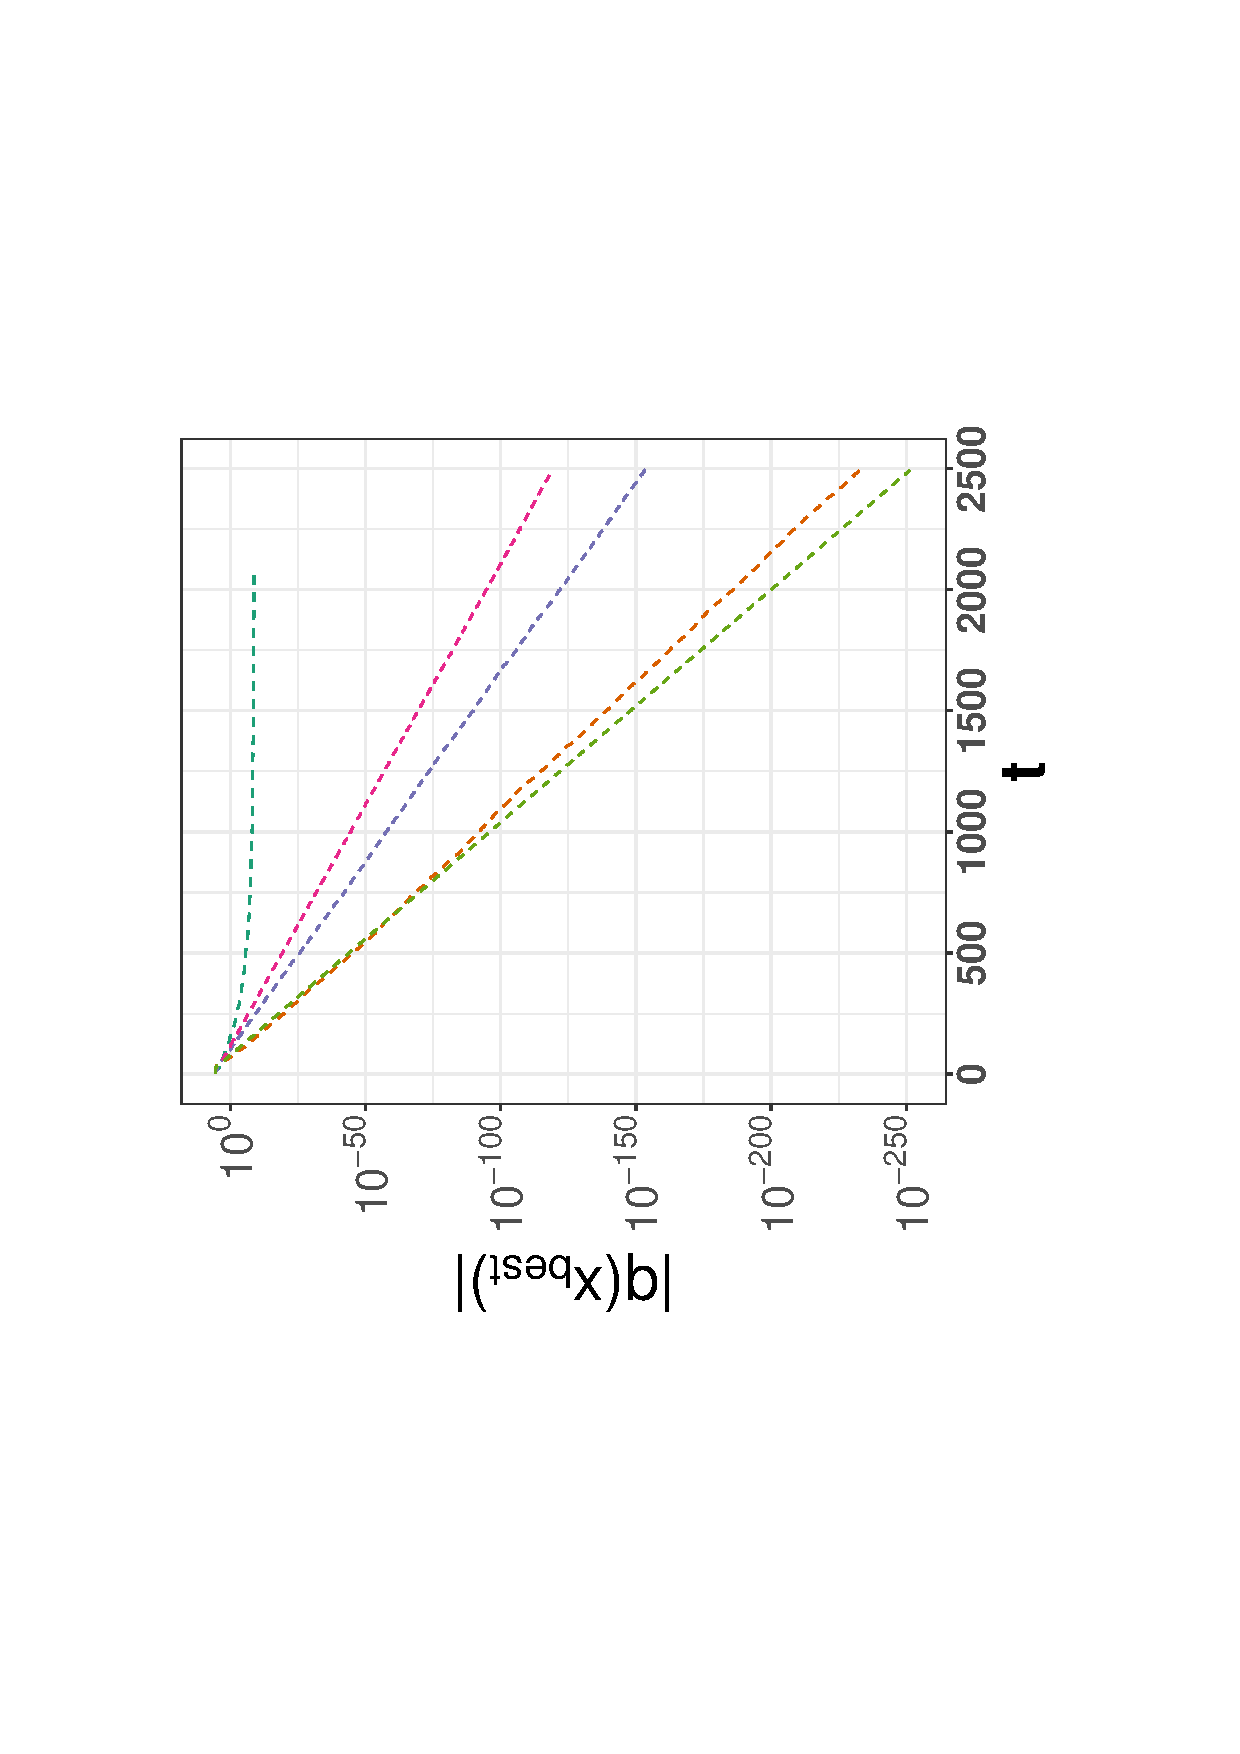
\includegraphics[width = 0.35\textwidth, angle = 270]{grid-sphere30}} 
\subfloat[]{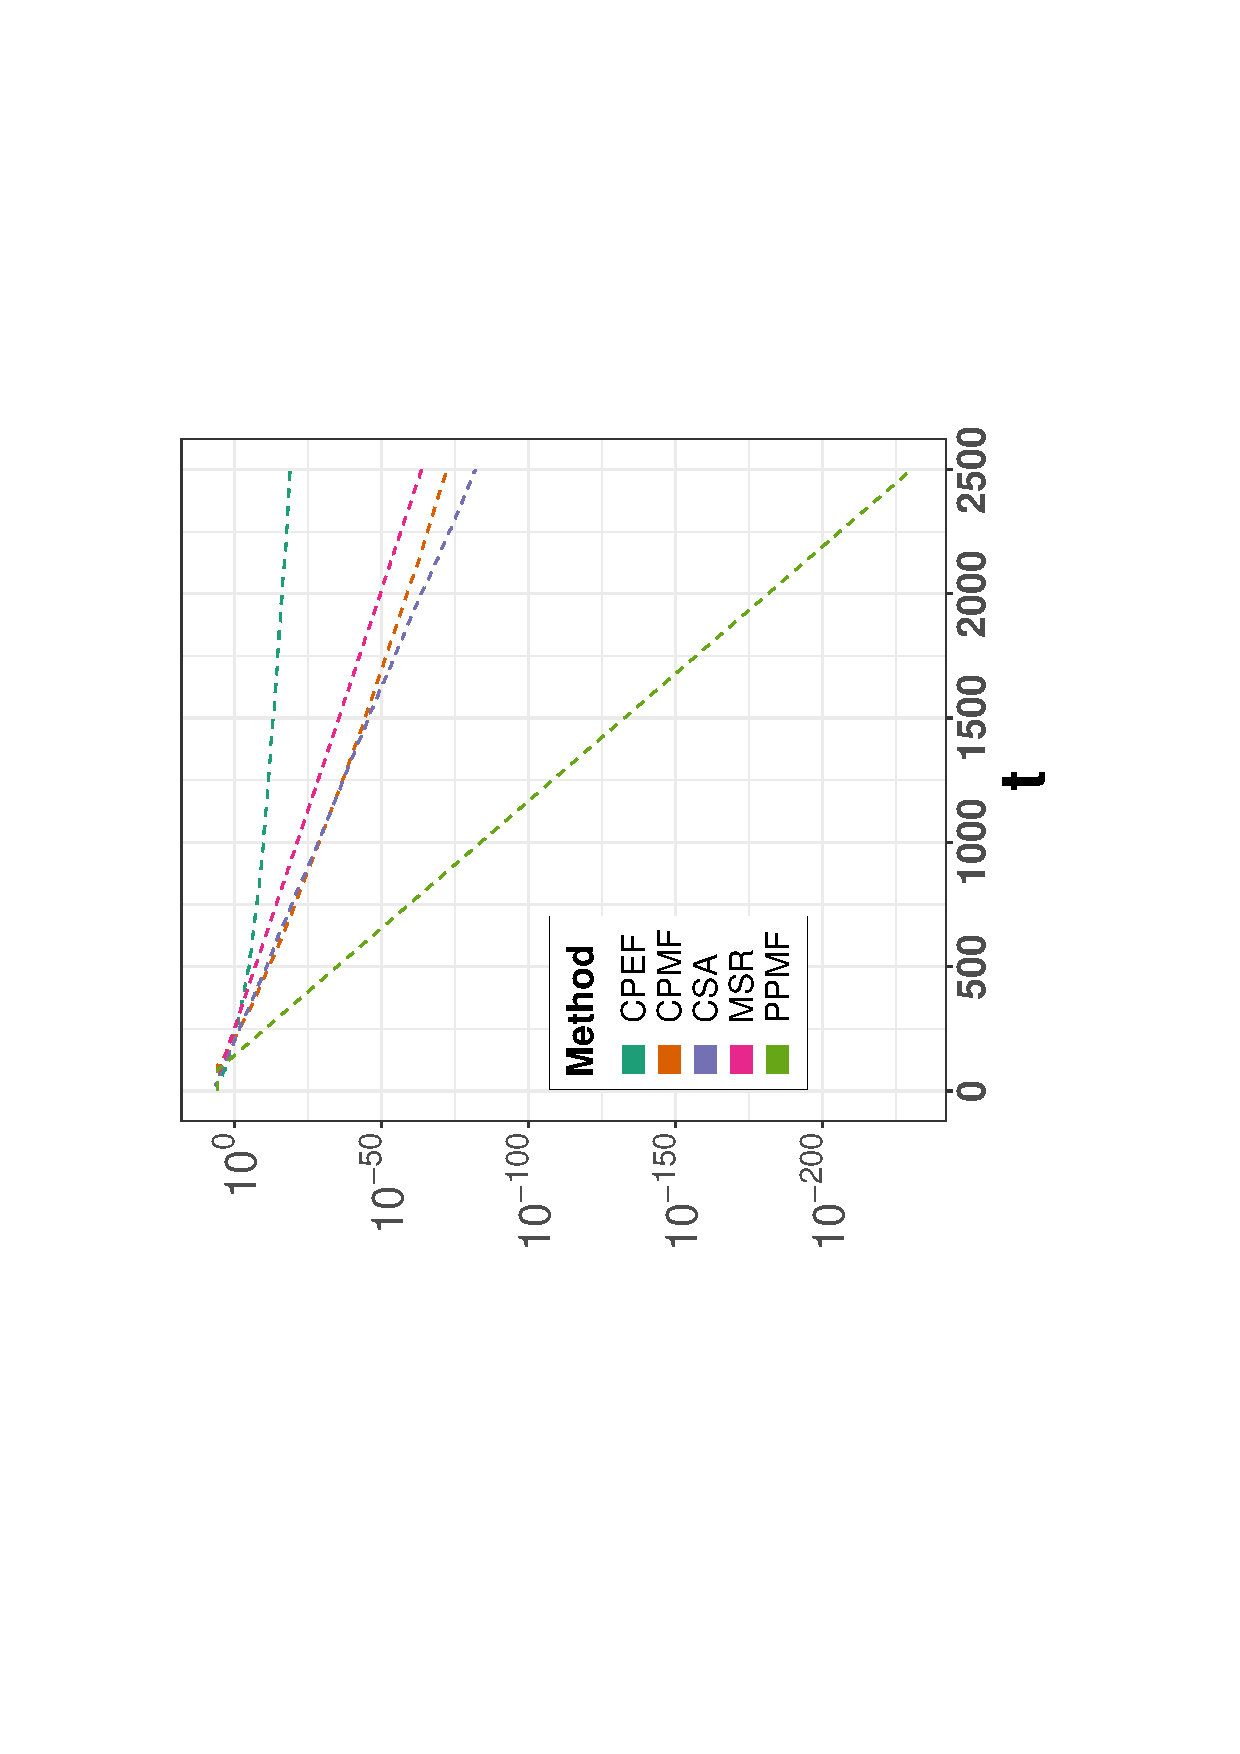
\includegraphics[width = 0.35\textwidth, angle = 270]{grid-sphere100}} \\
\subfloat[]{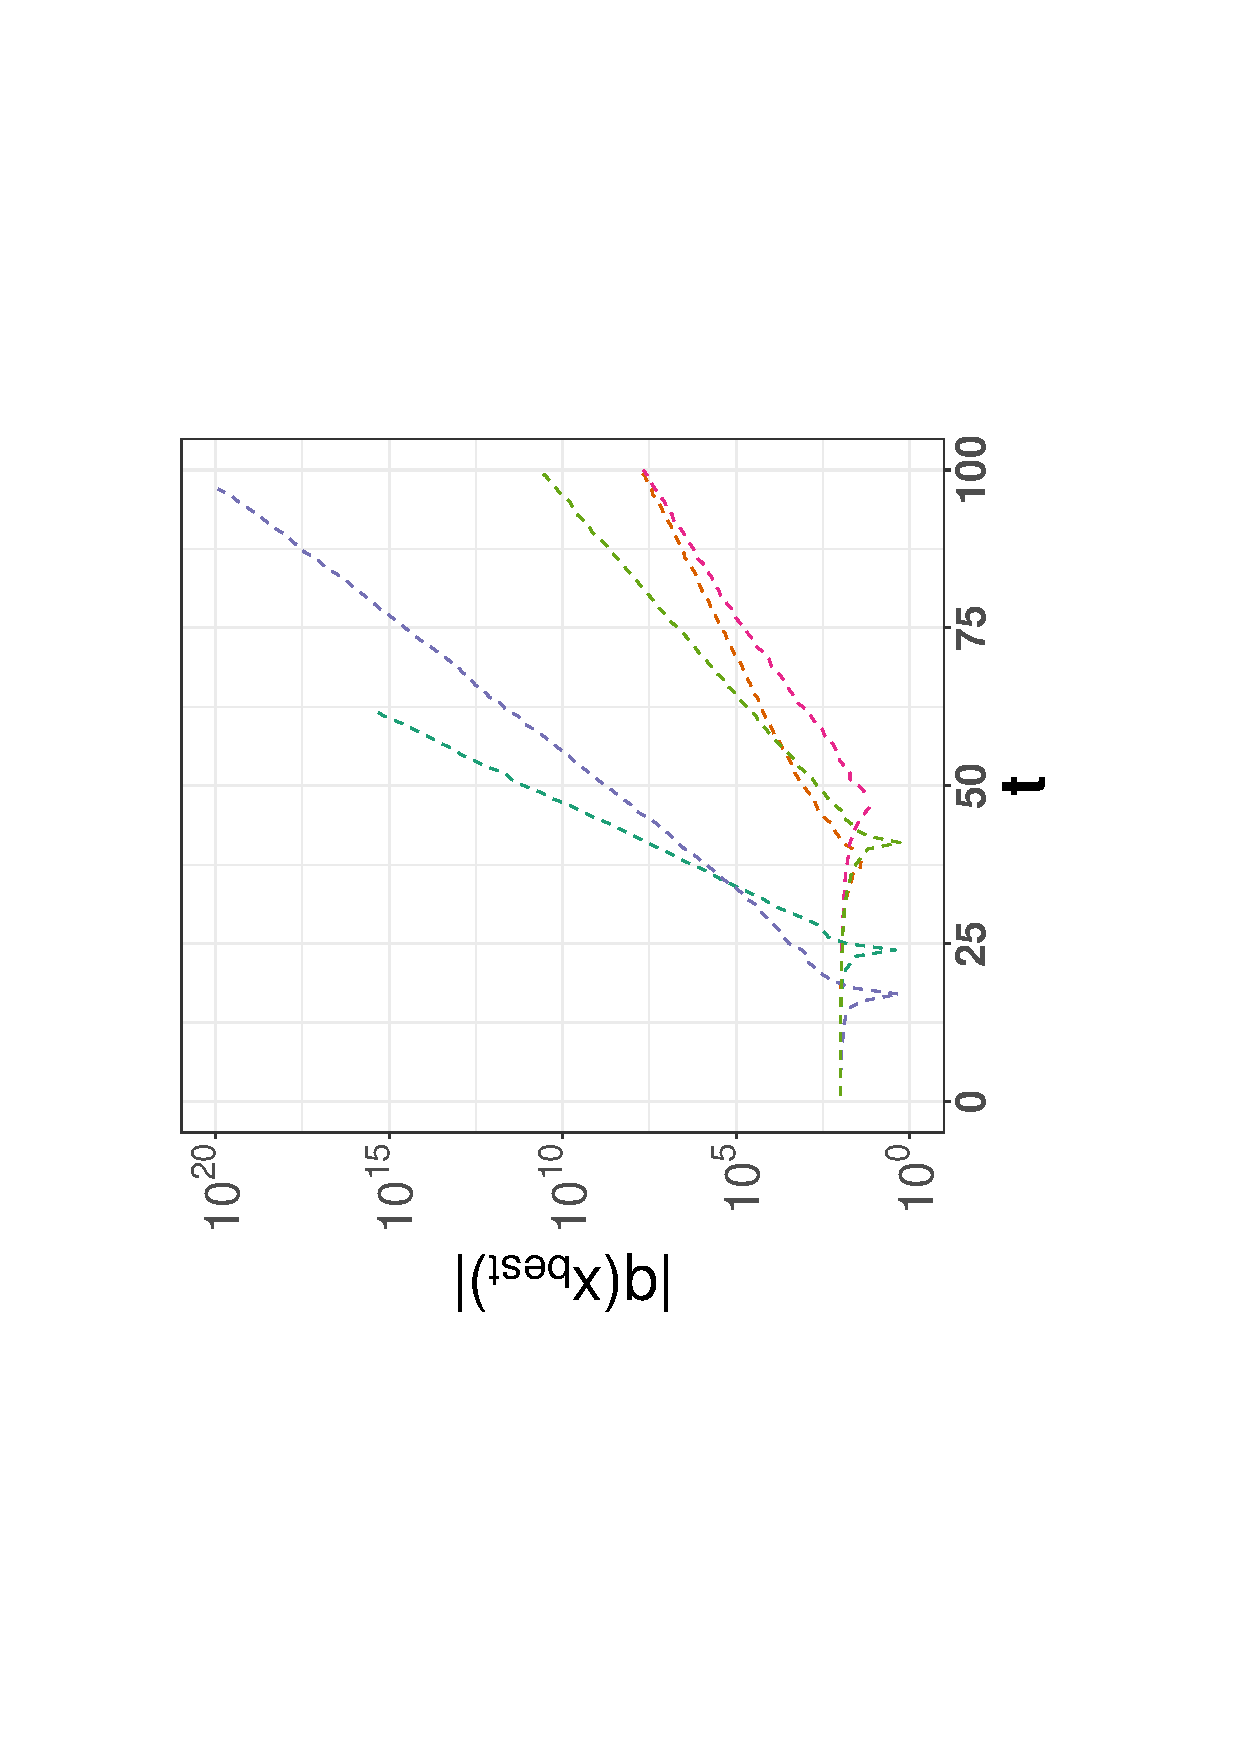
\includegraphics[width = 0.35\textwidth, angle = 270]{grid-linear30}} 
\subfloat[]{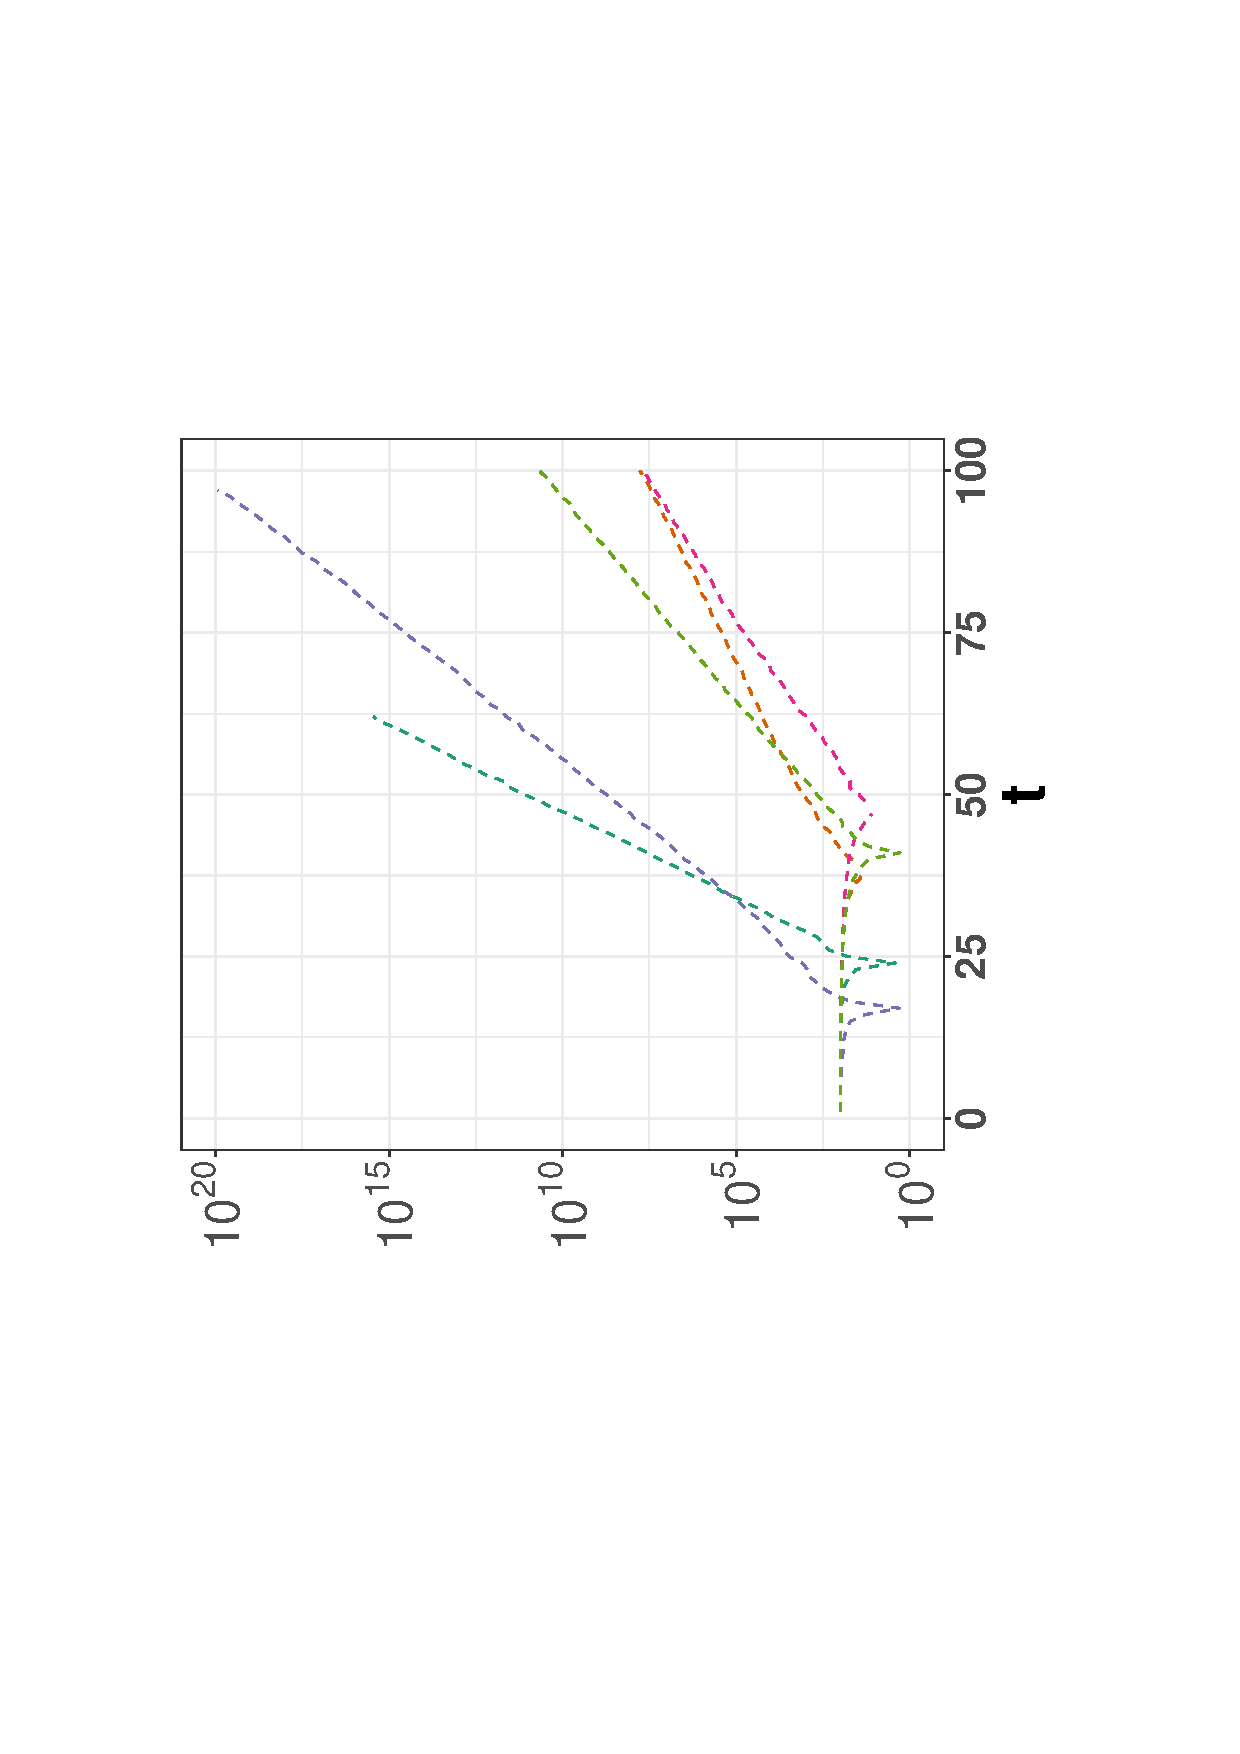
\includegraphics[width = 0.35\textwidth, angle = 270]{grid-linear100}} 
  \caption{Convergence curves for different fitness landscapes}.
\label{some example}
\end{figure}
